\documentclass[12pt]{article}
\usepackage{amsfonts} 
\usepackage[margin=0.8in]{geometry}
\usepackage[utf8]{inputenc}
\addtolength{\topmargin}{-.175in}
\usepackage{xcolor}
\usepackage{listings}
\usepackage{color}
\usepackage{graphicx}
\usepackage{wrapfig}
%\usepackage{lipsum}
\usepackage{subcaption}


\definecolor{dkgreen}{rgb}{0,0.6,0}
\definecolor{gray}{rgb}{0.5,0.5,0.5}
\definecolor{mauve}{rgb}{0.58,0,0.82}

\lstset{frame=tb,
language=python,
aboveskip=3mm,
belowskip=3mm,
showstringspaces=false,
columns=flexible,
basicstyle={\small\ttfamily},
numbers=none,
numberstyle=\tiny\color{gray},
keywordstyle=\color{blue},
commentstyle=\color{dkgreen},
stringstyle=\color{mauve},
breaklines=true,
breakatwhitespace=true,
tabsize=3
}


\author{{\Large Jonas Berggren, Jacob Maxton}}
\font\myfont=cmr12 at 30pt
\title{{\myfont Ökosystemsimulation}}

\begin{document}
\maketitle
\begin{abstract}
In diesem Dokument erklären wir, wie wir versucht haben eine numerische Simulation eines Ökosystems zu entwickeln, und was für Erkenntnisse sich daraus ziehen lassen.
Ausserdem gehen wir auf die Schwierigkeiten ein, auf die wir gestossen sind, und, wieso wir es nicht geschaft haben unsere ursprunglich beabsichtigten Ergnisse zu erhalten.
Unsere Simulation basiert auf Objektorientierter Programmierung und simuliert die Beute-Raueber-Beziehung zwischen Kaninchen und Fuechsen.
\end{abstract}
\tableofcontents
\newpage
\section{Die Simulation}
 \subsection{Objektorientierte Programmierung und numerischen Simulationen(Jonas)}
Objektorientierte Programmierung bezeichnet das Programmieren mit Hilfe so genannter Klassen und Objekte.
Ein Objekt, oder eine Instanz einer Klasse ist beispielsweise ein Individuum des Typs Kaninchen.
In dem Beispiel wuerde, die Klasse die Kaninchen im allgemeinen entsprechen.
Klassen kann man sich vorstellen wie Methodenkarten, in denen eine Reihe von Informationen gespeichert sind.
Diese koennen Instanzvariablen oder Methoden sein.
Instanzvariablen sind Variablen die jede Instanz traegt.
Methoden sind Funktionen oder Anweisungen die jede Instanz der Klasse ausfuehren kann.
Klassen haben ausserdem Hierarchien.
Eine Instanz einer sogenannten Unterklasse hat automatisch alle Methoden der uebergeordneten Klasse.
In unserer Simulation sind die Klassen \colorbox{gray!40}{Rabbit} und
\colorbox{gray!40}{Fox} Unterklassen zu \colorbox{gray!40}{Animal}.
Somit erben sie alle Methoden und Variablen von \colorbox{gray!40}{Animal}.

Bei numerischen Simulationen wird ein Szenario aus der reellen Welt durch eine Computersimulation nachgestellt.
Dabei wird das System zum Zeitpunkt $t$ betrachtet.
Auf Grundlage dessen wird der Zustand des Systems zum Zeitpunkt $t + h$ berechnet.
Dabei gilt, je kleiner $h$ ist, desto genauer ist die Simulation.
Alle aenderungen werden angewand und der Prozess wird wiederholt bis der gesamte Zeitraum Simuliert wurde, den es zu betrachten gilt.
Dies ist nuetzlich um die Gultigkeit von Modellen zu pruefen oder z.b. die Stabilitaet des betrachteten Systems zu testen.
\subsection{Konzept der Simulation(Jonas)}
In der Simulation werden Pflanzen Kaninchen und Fuechse simuliert.
Jedes Tier ist entweder eine Instanz der Klasse \colorbox{gray!40}{Fox} oder
\colorbox{gray!40}{Rabbit}, die jeweils Unterklassen der Klasse
\colorbox{gray!40}{Animal} sind.
In Animal sind alle Methoden gespeichert, die fuer Kaninchen und Fuechse
identisch ausgefuehrt werden, wie der Konstruktor
\colorbox{gray!40}{\_\_init\_\_} oder \colorbox{gray!40}{movetargeted} zum gezielten bewegen.
Methoden die fuer Fuechse und Kaninchen unterschiedlich sind, sind in den
jeweiligen Unterklassen gespeichert.
Diese sind z.b. \colorbox{gray!40}{findtarget}, zum finden aller potentiellen Ziele.
Auf die unterschiedlichen Instanzvariablen und Methoden wird aber in Kapitel \ref{methoden} weiter eingegangen.
Alle Tiere haben ein kreisförmiges Sichtfeld, was nicht die komplette Karte abdeckt.
Sie haben alle ein, mit der Zeit zunehmendes, Bedürfnis sich fortzupflanzen und zu essen.
Alle Bedürfnis werden bei deren Erfüllung verringert.
Wird der Hunger zu stark kann das Tier verhungern und sterben.
Ausserdem kann ein Tier zu jedem Zeitpunkt, mit einer Wahrscheinlichkeit sterben, die vom alter abhaengig ist.
Kaninchen essen pflanzen und Füchse essen Kaninchen, wobei gegessen Kaninchen sterben.
Kaninchen koennen vor Fuechsen fluechten die sich innerhalb des Sichtfelds befinden.

\subsection{Methoden(Jonas)}
\label{methoden}
\subsubsection{Aussuchen eines Ziels}
Dies wird durch die Methode \colorbox{gray!40}{findtarget} geregelt, die aus der Hauptschleife aufgerufen wird.
\colorbox{gray!40}{findtarget} ist sowohl eine Methode der Klasse
\colorbox{gray!40}{Fox} als auch der Klasse \colorbox{gray!40}{Rabbit}.
Dort sind sie aber unterschiedlich definiert, dar Fuechse sich anders verhalten sollen als Kaninchen.
Fuechse betrachten nur andere Tiere und speichern alle geeigneten Parnter in die Liste der Partner, und alle Kaninchen in die Liste der Potentiellen Malzeiten.
Kaninchen betrachten aber Tiere und Pflanzen.
Pflanzen werden zu essen gespeichert, Potenteille Partner zu Partnern und Fuechse zu Fluchtpunkten.
Objekte werden jedoch nur gespeichert wenn sie sich innnerhalb des Sichtradius \colorbox{gray!40}{self.sens} befinden.
Anschliessend wird geprueft welches Ziel angesteuert werden soll.
Dazu wird aus jeder Liste das naechste Element gesucht.
Wenn ein Kaninchen ein Fuchs sieht hat die Flucht immer oberste Priorität.
Der Fuchs wir anvisiert und der Bewegungsvektor wird mit -1 multipliziert.
Danach wird geprueft ob Hunger oder Libodo staerker wirkt und demnach wir
entschieden ob das naechste essen oder der naechste Partner anvisiert wird.

\subsubsection{Bewegung}
Die Bewegung der Tiere wird durch die Methoden \colorbox{gray!40}{movetargeted}
und \colorbox{gray!40}{moverandom} definiert.
Jedes Tier hat zwei Arten wie es sich fortbewegen kann.
Wenn es ein bestimmtes Ziel hat, wird \colorbox{gray!40}{movetargeted}
aufgerufen, und das Tier bewegt sich entlang des Vektors von der eigenen Position zum Ziel.
Dabei ist der Bewegungsvektor auf die Bewegungsgeschwindigkeit normiert.
Wenn kein Ziel in Sicht ist, wird \colorbox{gray!40}{moverandom} aufgerufen, und sie bewegen sich zufällig.
In beiden Faellen wird die Methode \colorbox{gray!40}{collision} jedes mal aufgerufen.
Diese verhindert das Tiere aus der Karte raus laufen.
\subsubsection{Fortpflanzung und Mutation}
Es koennen nur gleichrassige, heterosexuelle und altersgerechte Paare ein Kind zeugen.
Ausserdem mussen beide Eltern fuer ein bestimmten Zeit keiner Kinder gezeugt haben, und sie duerfen fuer eine Laengere Zeit nicht mit einander Kinder gezeugt haben.
Haben sich zwei gefunden wird der Liste der Tiere eine neue Instanz der Klasse hinzugefügt.
Fuer die Definition der mutierbaren  Eigenschaften wird der Durchschnitt aus den jeweiligen Werten der Eltern als Mittelwert angenommen.
Der Wert des Kindes weicht um $x$ von diesen Durchschnitt ab, wobei $x$ eine zufaellige Zahl zwischen $-0.1$ und $0.1$ ist.

Die Eltern speichern sich gegenseitig als ehemalige Partner ab und betrachten
sich anschließen für eine festgelegte Frist nicht mehr als mögliche Partner. 
\subsubsection{Tod}
Tiere koennen auf drei untertschiedlichen Arten sterben.
Sie koennen verhungern, sie koennen durch die Altersabhaengige Funktion sterben
oder Kaninchen koennen gefressen werden.
Dies wird durch die Methoden \colorbox{gray!40}{starve}, \colorbox{gray!40}{die}
und \colorbox{gray!40}{eat} geregelt.
Die Methoden \colorbox{gray!40}{starve} und \colorbox{gray!40}{die} werden bei
jeder Iteration aufgerufen, und \colorbox{gray!40}{eat} wenn ein Kaninchen gefressen wird.
%starve

Die Todeswahrscheinlichkeitsdichte wird durch eine Funktion beschrieben nach dem Muster:
\begin{equation}
    P = a ( {e}^{-t + b} \cdot c \cdot t + d)
    %val = 0.0000001*(e**(-1.0*(self.age)+4.8)+20.0*self.age-4.0)
\end{equation}

Der Graf zeigt die Todeswarscheinlichkeitsdichte um eine Groessenordnung vergoessert.
\begin{figure}[h!]
  \centering
  \begin{subfigure}[b]{0.4\linewidth}
    \includegraphics[width=\linewidth]{Screenshot_2019-12-20 Grafikrechner - GeoGebra(1).png}
  \end{subfigure}
  \begin{subfigure}[b]{0.4\linewidth}
    \includegraphics[width=\linewidth]{Screenshot_2019-12-20 Grafikrechner - GeoGebra(2).png}
  \end{subfigure}
  \caption{Todeswahrscheinlichkeitsdichte}
  \label{fig:coffee}
\end{figure}
\newpage
Durch so eine Funktion ist P fuer ein kleines t relativ gross.
P erreicht im positiven Wertebereich ein Minimum und waechst dann approximativ linear an.
Dies fasst Kindersterblichkeit und Alterschwaeche in ein Funktion zusammen.
Die Funktion P kann Werte Annehme dei groesser sind als 1.
Das ist aber aufgrund der Funktionsweise des Prgramms nicht problematsich.
Beim sterben durch gegessen werden loescht der Fuchs die gegessene Instanz aus der Liste der Tiere.
\subsubsection{Andere Methoden}
Hinzu kommen noch weiter Hifsmethoden wie z.b. \colorbox{gray!40}{distance}, die
den Abstand zwischen self und einem beliebigen Punkt berechnet.
Diese sind jedoch fuer das allgemeine Verstaendniss unsere Abreit nicht essentiell.
\subsection{Frontend (Jacob)}
Was bringt die beste Simulation, ohne dass man sich die Werte angucken kann? Gar
nichts. Deswegen haben wir 4 Dateien, die automatisch von dem Script in einem Ordner
zusammengefasst werden:

 Log.txt

Die Log.txt ist eine Textdatei die, oh wie wunder, den Log der Simulation enthält.
Hier wir immer wenn ein Tier stirbt, ein neuer Tag beginnt oder irgendetwas anderes
Passiert, dies in eine neue Zeile eingetragen. Dies sorgt für eine unglaublich große
Datei, die vor allem mit kurzen Zeilen gefüllt ist. Deswegen will man sich als
Mensch diese Datei nur angucken müssen, wenn man unbedingt muss. Muss man
aber nicht, da die wichtigen Informationen auch in den anderen Dateien Stehen:

Info.txt
    
    Info.txt ist schon wieder eine Textdatei, aber diesmal eine deutlich kürzere:
        Die Info.txt hat nur 5 Zeilen: Eine Datei, die die Laufzeit (die Anzahl der Tage der
        Simulation), sowie die Anzahl und Gründe der Todesfälle nach Tierart gegliedert
        auflistet. So kann man aus dieser Datei genau auslesen, wie viele Füchse im Laufe
        der Simulation an Hunger gestorben sind, oder wie viele Hasen von Füchsen
gefressen wurden.
\newpage
\begin{wrapfigure}{h}{0.5\textwidth}
        \centering
        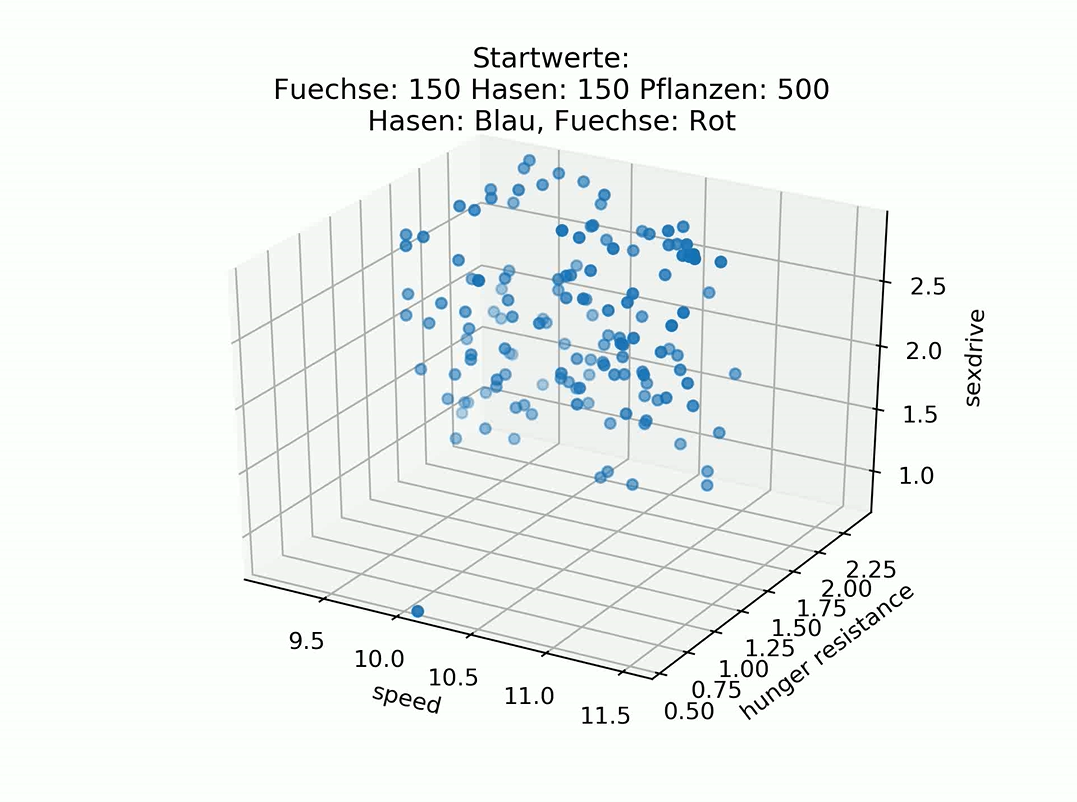
\includegraphics[width=0.5\textwidth]{stillframe.PNG}
        \caption{Lotka-Volterra-Regeln \label{overflow}}
\end{wrapfigure}

Viel einfacher für den Menschen anzuschauen sind jedoch die beiden Videos, kreativ
    benannt: video.avi und video2.avi.
        Video.avi ist hier eine Videodatei, die eine Zeitliche auflösung der Mutationenen
        aufzeigt: Hier werden Dreidimensionale Graphen dargestellt, auf jeder der Achsen
        jeweils einer der Werte, die wir mutieren:
        Geschwindigkeit, Hungerresistenz und ein
        Skalar für den Sexualtrieb. Diese sehen ungefähr
        so aus:
        Hier können wir eine sehr frische Zivilisation
        sehen; die Werte entsprechen noch sehr den
        Ursprünglichen Werten. Wir können an diesen
        Graphen auch auslesen, dass die geringste
        Hungerresistenz, die jemals bei einem Tier in
        dieser Simulaiton vorhanden war 0.5 ist. Dies
        erkennt man, da Ober- und Untergrenzen der
        Achsen so gesetzt sind, dass die geringsten und größten innerhalb einer Simulation
        verzeichneten Werte die Ober- und Untergrenzen festlegen. Das liegt daran, dass in
        dem Video 15 Graphen pro Sekunde zu einem Video zusammengeschnitten sind, und
        diese andernfalls unlesbar wären.
        Ähnlich ist auch video2.avi, welches eine Visuelle Repräsentation der Simulation
        darstellt. Die Punkte, die sich nicht bewegen, sind hier Pflanzen, die dunklen
        bewegenden Punkte Hasen und die Hellen bewegenden Punkte Füchse. Auch dieses
        Video ist mit 15 fps gerendert, und weil ein Bild jeweils einem Tag entspricht
        werden in den Videos also immer 15 Tage pro Sekunde dargestellt.

\section{Die Analyse}
\subsection{Theorethisch}

\begin{wrapfigure}{r}{0.5\textwidth}
        \centering
        \includegraphics[width=0.5\textwidth]{LotkaVolterra.png}
        \caption{Lotka-Volterra-Regeln \label{overflow}}
\end{wrapfigure}
Uns ist es mit den Mitteln, die wir haben nicht gelungen Die Simulation so zu gestalten, dass es lange genung dauert bis eine der Tierarten austirbt, um daraus Erkenntnisse ziehen zu koennen.
Dies ist dadurch zu erklaeren, dass uns nicht gelungen ist ein Verhaeltnis von alle Parametern zu finden, was die Simulation haltbar macht.

In der Oekologie gelten so genannte Lotka-Volterra-Regeln.
Diese sagen eine Periodische Oszillation der Populationen von Raub- und Beutetieren voraus.
Diese wird durch das Narhungsangebot fuer die Raeuber sowie, das Risiko gegessen zu werden fuer die Beutetiere, verursacht.
Uns ist es nicht gelungen unsere Werte so anzupassen, dass das Minimum dieser Oszilation ueber 0 bleibt.
Oekosysteme haben eine sehr heikle Ballance.
Ins besondere Raeuber duerfen weder zu gute noch zu schlechte Jager sein, damit das System so bestehen bleiben kann.
Sind sie zu schnell, zu zahlreich, zu fortpflanzungsfahig, zu hungerresistent, etc. besteht schnell das Risiko, dass sie ihrer Beutetiere ausrotten und somit sich selbst.
Sind sie in diesen Eigenschaften zu schwach koennen sie auch mit umfangreichem Essens Angebot nicht ueberleben.
Deswegen ist die Vielfalt von okosystemen so wichtig fuer deren Fortbestand.

\subsection{Praktisch}
Warum haben wir unser Ziel nicht erreicht? Wie Jonas schon ausgeführt hat ist es sehr
kompliziert, die richtigen Werte zu finden. Was man also machen müsste ist, sehr viele
Werte auszuprobieren. Hier kommen jedoch viele Probleme auf informatischer Seite:
Zeit. Es dreht sich alles um Zeit. Jeder Tag einer Simulation dauert im schnitt 0.1 bis 0.4
Sekunden, zur Vorrechnung werde ich den Wert 0.1 benutzen. Da jede Simulation auf
grundlegendem Zufall basiert (bei der Bewegung, Mutation etc.), müssen wir also
mehrere Simulationen mit den gleichen Werten machen, und die Mittelwerte nehmen,
damit wir sicher sagen können, dass eine wertekombination wirklich gut ist, und nicht
einfach nur durch Zufall lange angehalten hat. Mein Computer kann gleichzeitig 3Simulationen laufen lassen kann (er hat 4 Kerne, also eine Simulation pro Kern und ein
Kern für die Kontrolle und Verarbeitung der Informationen), deswegen haben wir pro
Werte jeweils 5 Simulationen gemacht, dadurch konnten wir den Fehler durch den Zufall
zufriedenstellend beheben, ohne die Zeit pro Wertekombination in die Länge zu ziehen.
Das führt dazu, dass jeder Tag in diesen Simulationen letztendlich 0.2 bis 0.8 Sekunden
braucht, da ja nicht nur eine Simulation, sondern 5 Simulationen berechnet werden
müssen, davon jedoch nur 3 gleichzeitig. Zwei Kerne können nicht an der selben
Simulation rechnen.
Machen wir also eine einfache Rechnung: Gehen wir von einer durchschnittlichen
Laufzeit von 100 Tagen aus. Dann brauchen wir, um jeweils eine Wertekombination zu
testen: 100 * 0,2s = 20s oder, mit dem Größeren Wert, 100 * 0,8s = 80s. Dieser Wert ist
für ein Wertepaar. Und jetzt kommt das Problem: Wir wissen nicht, welche Werte gut
sind, und welche schlecht. Wir müssen den Computer also raten lassen. Aber wenn jetzt
jeder Wert 50 Sekunden (Mittelwert zwischen 20 und 80) dauert, dann sind das mit den
Schritten dass der Teste-Script auch noch erkennen muss, ob das gerade gut oder
schlecht war, eine Minute pro Wertekombination. Und damit schaffen wir 60
Wertekombinationen pro Stunde-einfach Raten geht also nicht.
Nehmen wir also einen Ansatz aus der AI-Technologie: Machine Learning, genauer:
einen Genetic Algorytm. Dieser nimmt letztendlich die beiden besten
Wertekombinationen, die er hat, und bastelt aus den beiden ein neues Wertepaar. Dieses
wird nun mit einer geringen Wahrscheinlichkeit um einen geringen Wert abgeändert, und
getestet. Danach beginnt das ganze von Vorne. Theoretisch ist dieser Anlauf ein sehr
guter, und führte bei meinen anderen Anwendungen auch schon mehrfach zu
erfolgreichen AIs. Was ich hier nicht bedacht hatte: Genetic Algorythms brauchen
tausende generationen, um wirklich ein gutes Ergebnis zu liefern. Und auch nur
eintausend Generationen laufen zu lassen hat bei unseren Geschwindigkeiten 12 Stunden
gebraucht. Noch dazu ist eine Simulation auszutarieren eine sehr komplizierte Aufgabe.
Als Vergleich: Eine AI zu schreiben, und zu trainieren, die Minesweeper Spielt (eine
sehr leichte Aufgabe) hatte bei mir mit einem Genetic Algorythm 14.000 Generationen
gebraucht, bis es das hinbekommen hat – dank einer Effizienteren Programmsprache und
eines einfacheren Problems habe ich damals aber 500 generationen pro Minute
hinbekommen. Bei der Simulation erwarte ich also (im Nachhinein) sogar sechsstellige
Generationenzahlen, was (mit dem Wert der Minute Pro Simulaiton) 69,4 Tage dauern
würde. Diese Zahl ist wahrscheinlich sogar sehr optimistisch, da mit besseren Werten die
Simulationen länger dauern würden, und die maximale Länge der Simulationen auf
10.000 Tage festgelegt ist. Es war also von Anfang an unmöglich, die Simulation auf die
Art und Weise, wie wir sie gemacht haben, so auszutarieren, dass wir werte haben, mit
denen wir eine Population haben, die überhaupt überlebensfähig ist. Und erst, wenn
nicht alle 500 Hasen in den ersten 10 Tagen sterben, können wir untersuchen, wie sich
die Hasen verändern, wenn wir z.B. mehr Füchse haben, oder weniger Essen.


\section{Verbesserungsmoeglichkeiten (Jonas)}
Eine Moeglichkeit das Programm zu verbessern waere ein sogenanntes Gridsystem zu implementieren.
Dabei wird das Feld in mehrere Subfelder unterteilt.
Die Objekte werden in einer Matrix gespeichert wobei jeder Index der Matrix eine Subfeld zugeordnet ist.
Das bietet den Vorteil, dass die Tiere bei Jeder Iteration nicht mehr die Die
Position aller Objekte abfragen muessen, sondern nur die der Objekte die sich im
selben bzw. in einem der Felder befinden, die mit dem Sichtkreis ueberlappen.
Somit kann die Laufzeit pro Iteration stark reduziert werden.

Asserdem kann eine andere, schnellere Programmiersprache verwendet werden.
Fuer Umfangreiche wissenschaftliche Anwendungen kann eine erweiterte Version
eines solchen Programms auf staerkeren Computern ausgefuehrt werden.
\section{Anwendungen}
Eine Umfangreichere Simulation dieser Art koennte nuetzlich sein um die Auswirkungen von Menschlichem Eingriff in oekosysteme wie Klimaerwaermung, Lebensraum veraendungen oder austerben einer Art abzuschaetzen.
Dies koennte nuetzlich sein um Notwendigkeit und Dringlichkeit von Umwelt Massnahmem abzuschaetzen.
\section{Fazit}
Wir haben mit Hilfe Objektientierter Programmierung eine Vereinfachte Simulation
eines OEkosysteme entwickelt indem wir uns auf die Wechselwirkung zwischen zwei Tierarten konzentriert haben.
Dabei sind wir auf unterschiedliche Schwierigkeiten gestossen.
Zuerst mussten wir entscheiden wie genau unsere Simulation sein soll.
Anschliesend war es sehr schwierig all Willkuerrlich gewaehlten Parameter so zu beziffern, dass keine der Arten zu schnell ausstrirbt.
Dabei haben wir festgestellt wie fragil auch so ein einfaches OEkosystem sein kann.
\end{document}
